%%%%%%%%%%%%%%%%%%%%%%%%%%%%%%%%%%%%%%%%%
% a0poster Portrait Poster
% LaTeX Template
% Version 1.0 (22/06/13)
%
% The a0poster class was created by:
% Gerlinde Kettl and Matthias Weiser (tex@kettl.de)
% 
% This template has been downloaded from:
% http://www.LaTeXTemplates.com
%
% License:
% CC BY-NC-SA 3.0 (http://creativecommons.org/licenses/by-nc-sa/3.0/)
%
%%%%%%%%%%%%%%%%%%%%%%%%%%%%%%%%%%%%%%%%%

%----------------------------------------------------------------------------------------
%	PACKAGES AND OTHER DOCUMENT CONFIGURATIONS
%----------------------------------------------------------------------------------------

\documentclass[a0,portrait]{a0poster}

\usepackage{multicol} % This is so we can have multiple columns of text side-by-side
\columnsep=100pt % This is the amount of white space between the columns in the poster
\columnseprule=3pt % This is the thickness of the black line between the columns in the poster

\usepackage[svgnames]{xcolor} % Specify colors by their 'svgnames', for a full list of all colors available see here: http://www.latextemplates.com/svgnames-colors

\usepackage{times} % Use the times font
%\usepackage{palatino} % Uncomment to use the Palatino font

\usepackage{graphicx} % Required for including images
\graphicspath{{figures/}} % Location of the graphics files
\usepackage{booktabs} % Top and bottom rules for table
\usepackage[font=small,labelfont=bf]{caption} % Required for specifying captions to tables and figures
\usepackage{amsfonts, amsmath, amsthm, amssymb} % For math fonts, symbols and environments
\usepackage{wrapfig} % Allows wrapping text around tables and figures
\usepackage{subfig}
\usepackage{lipsum}
\usepackage{hyperref}

\begin{document}

%----------------------------------------------------------------------------------------
%	POSTER HEADER 
%----------------------------------------------------------------------------------------

% The header is divided into two boxes:
% The first is 75% wide and houses the title, subtitle, names, university/organization and contact information
% The second is 25% wide and houses a logo for your university/organization or a photo of you
% The widths of these boxes can be easily edited to accommodate your content as you see fit

\begin{minipage}[b]{0.75\linewidth}
%\veryHuge \color{NavyBlue} \textbf{HERA-19} \color{Black}\\ % Title
%\Huge\textit{Commissioning}\\[2cm] % Subtitle
\veryHuge \color{NavyBlue} \textbf{The sky seen by HERA 19} \color{Black}\\ % Title
\\
\huge \textbf{T.L.~Grobler}\\[0.5cm] % Author(s)
\\
\huge Rhodes University, Department of Physics and Electronics\\[0.4cm] % University/organization
%\Large \texttt{john@LaTeXTemplates.com} --- 1 (000) 111 1111\\
\end{minipage}
%
\begin{minipage}[b]{0.25\linewidth}

\includegraphics[width=20cm]{Rhodes_logo.jpg}\\
\end{minipage}

\vspace{1cm} % A bit of extra whitespace between the header and poster content

%----------------------------------------------------------------------------------------

\begin{multicols}{2} % This is how many columns your poster will be broken into, a portrait poster is generally split into 2 columns

%----------------------------------------------------------------------------------------
%	ABSTRACT
%----------------------------------------------------------------------------------------

\color{Navy} % Navy color for the abstract

\begin{abstract}
The Hydrogen Epoch of Reionization Array (HERA) is a low frequency (100-200 MHz), 350-dish radio interferometer currently under construction at the SKA site in the Karoo. Its main goal is to observe the evolution of the 21-cm line emitted by the intergalactic medium in the $6 < z < 12$ range, therefore providing a complete characterization of cosmic reionization. The first 19 dishes were deployed at the end of 2015. 
Here I present the results that we obtained after reducing three Julian days (2457545, 2457555 and 2457661) worth of HERA-19 snapshots using our own custom built commissioning pipeline. Each of the three Julian days that we processed
contained 72 ten minute snapshots.
\end{abstract}

\section{Scientific background}
The 21-cm emission from redshifted neutral Hydrogen is the most promising probe of the cosmic evolution of the intergalactic medium and its transition from the dark ages to cosmic reionization. The detection of the 21-cm signal has been the main driver of several radio interferometric array 


%\color{DarkSlateGray}





%----------------------------------------------------------------------------------------
%	INTRODUCTION
%----------------------------------------------------------------------------------------

%\color{SaddleBrown} % SaddleBrown color for the introduction

%\section*{Introduction}

%Aliquam non lacus dolor, \textit{a aliquam quam} \cite{Smith:2012qr}. Cum sociis natoque penatibus et magnis dis parturient montes, nascetur ridiculus mus. Nulla in nibh mauris. Donec vel ligula nisi, a lacinia arcu. Sed mi dui, malesuada vel consectetur et, egestas porta nisi. Sed eleifend pharetra dolor, et dapibus est vulputate eu. \textbf{Integer faucibus elementum felis vitae fringilla.} In hac habitasse platea dictumst. Duis tristique rutrum nisl, nec vulputate elit porta ut. Donec sodales sollicitudin turpis sed convallis. Etiam mauris ligula, blandit adipiscing condimentum eu, dapibus pellentesque risus.

%\textit{Aliquam auctor}, metus id ultrices porta, risus enim cursus sapien, quis iaculis sapien tortor sed odio. Mauris ante orci, euismod vitae tincidunt eu, porta ut neque. Aenean sapien est, viverra vel lacinia nec, venenatis eu nulla. Maecenas ut nunc nibh, et tempus libero. Aenean vitae risus ante. Pellentesque condimentum dui. Etiam sagittis purus non tellus tempor volutpat. Donec et dui non massa tristique adipiscing.

%----------------------------------------------------------------------------------------
%	OBJECTIVES
%----------------------------------------------------------------------------------------

\color{DarkSlateGray} % DarkSlateGray color for the rest of the content
\section*{Pipeline}

The basic HERA-19 pipeline that was implemented is shown in the flow diagram below. We mainly concentrate on how the calibration sub-blocks were implemented in this poster.  

\begin{center}\vspace{1cm}
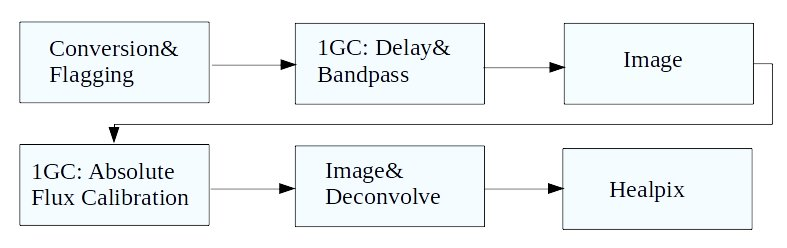
\includegraphics[width=0.8\linewidth]{pipeline.jpg}
\captionof{figure}{\color{Green} The custom built HERA-19 Pipeline. \url{https://github.com/Trienko/heracommissioning}.}
\end{center}\vspace{1cm}

An image of the HERA-19 array is shown below. 

\begin{minipage}{\columnwidth}
    \makeatletter
    \newcommand{\@captype}{figure}
    \makeatother
    \centering
    \subfloat[HERA-19 Image]{%
      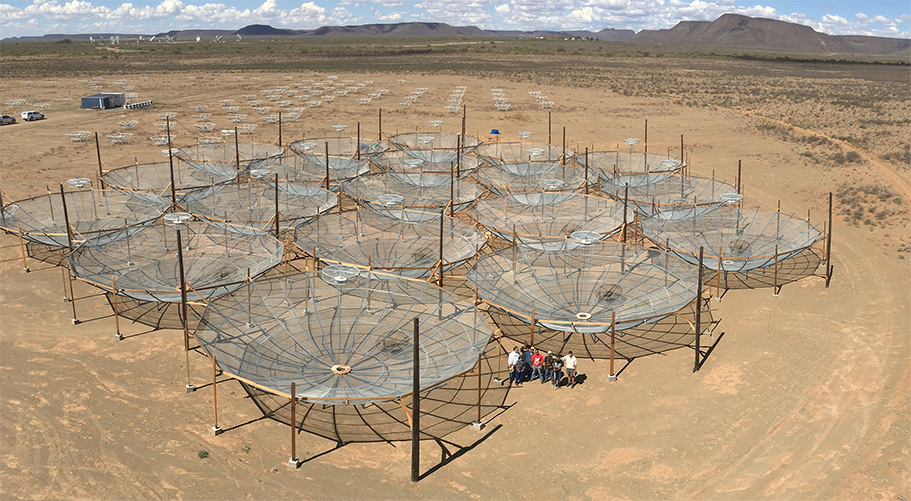
\includegraphics[width=0.47\linewidth]{hera19H.png}%
      \label{fig:evaluation:revenue}%
    }\qquad%
    \subfloat[HERA-19 Layout]{%
      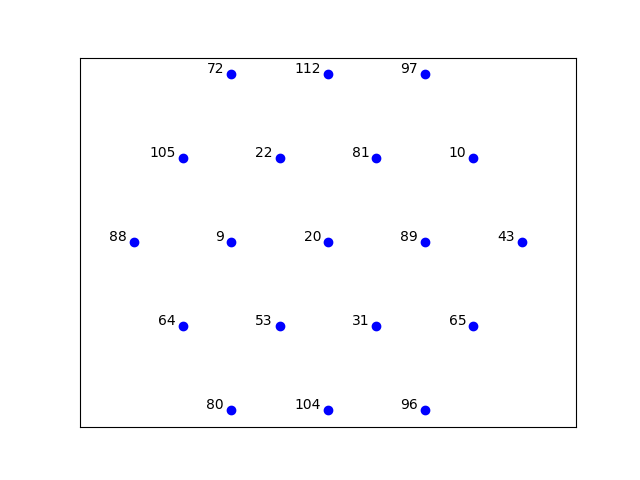
\includegraphics[width=0.4\linewidth]{Layout.png}%
      \label{fig:evaluation:avgPrice}%
    }
    \caption{\color{Green} HERA-19.}
  \end{minipage}

% \begin{center}\vspace{1cm}
% 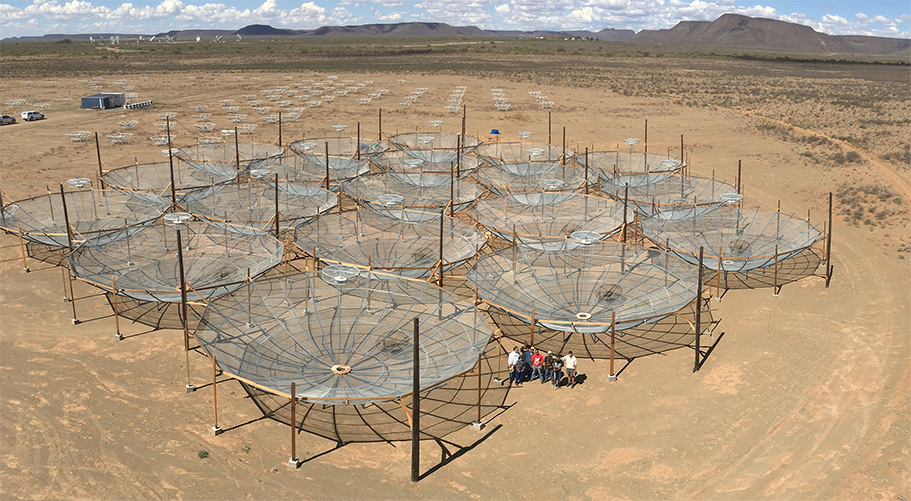
\includegraphics[width=0.6\linewidth]{hera19H.png}
% \captionof{figure}{\color{Green} An image of HERA-19.}
% \end{center}\vspace{1cm}
% \begin{center}\vspace{1cm}
% 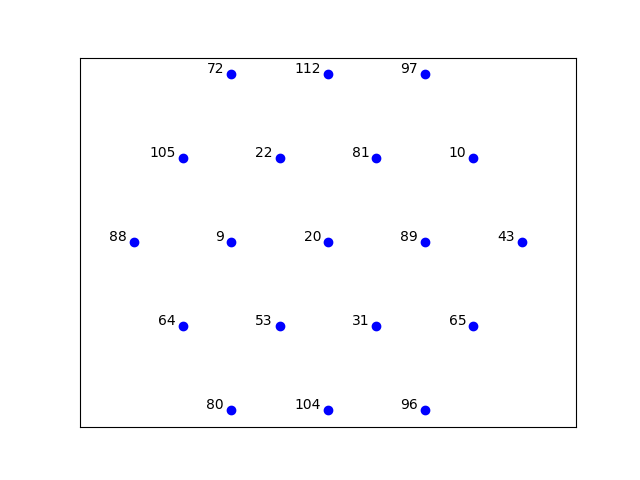
\includegraphics[width=0.6\linewidth]{Layout.png}
% \captionof{figure}{\color{Green} An image of HERA-19.}
% \end{center}\vspace{1cm}

\section*{Calibration}

%Our pipeline only includes a first generation calibration (1GC) step (i.e. we make use of calibrator sources). The calibration procedure we used consisted of a two stage process.
Due to the limited angular resolution of HERA-19, the Galactic centre is almost unresolved and can therefore be used to calibrate the array.
We selected the snapshot (i.e. 10 minute long) observation when the Galactic centre transits and model it as an unresolved 1~Jy source with a flat spectrum in the HERA-19 band. We calibrated by first determining the antenna--based delays using the CASA\footnote{http://casa.nrao.edu} task {\it gaincal}, thereafter we computed the complex gains as a function of frequency using the CASA task {\it bandpass} (Figure~\ref{fig:delays} and~\ref{fig:bandpass}).
\begin{center}\vspace{1cm}
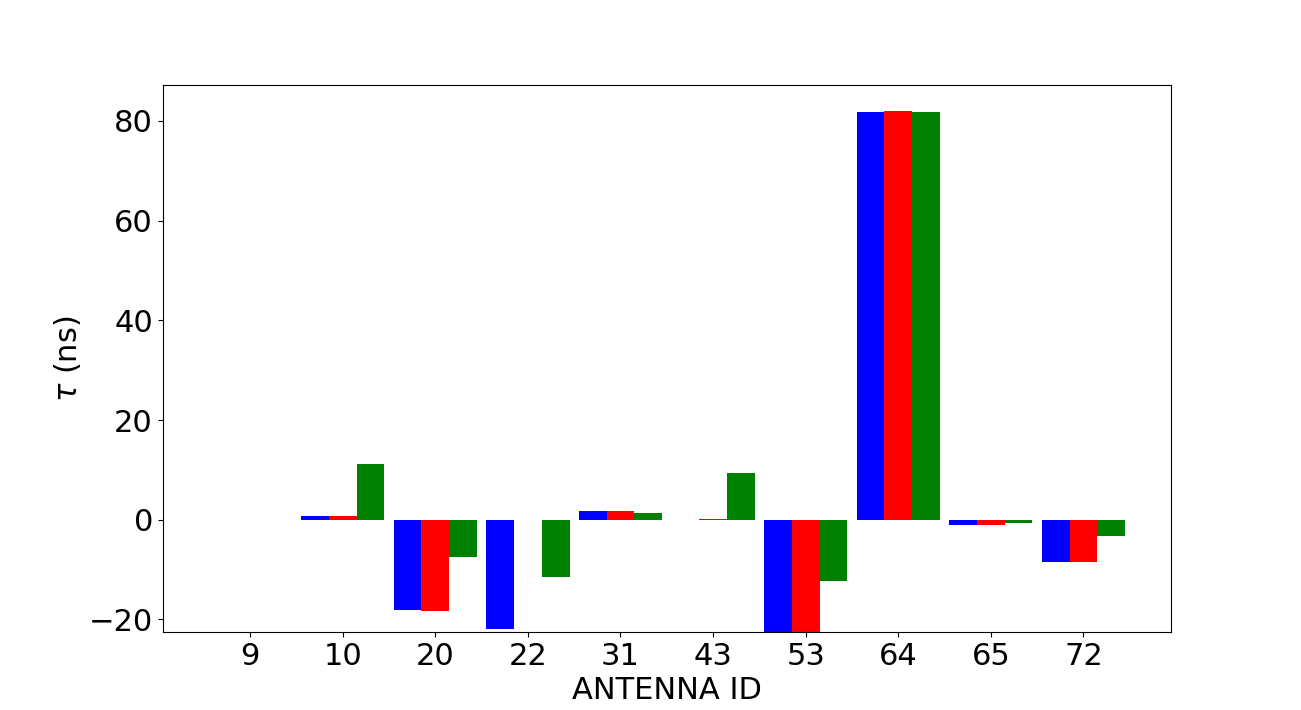
\includegraphics[width=0.8\linewidth]{delay.png}
\captionof{figure}{The computed delays. (\bf GB: I would remove the figure title. I would also remove the legend and write in the caption which day correspond to which colour. Rather than using JDs use the actual calendar day with time. I suggest to plot only till antenna 72 to make the plot less crowded, but all the antennas need three JD values or an explanation why not. It should be (ns) rather than [nsec]).}
\label{fig:delays}
\end{center}\vspace{1cm}
%
\begin{minipage}{\columnwidth}
    \makeatletter
    \newcommand{\@captype}{figure}
    \makeatother
    \centering
    \subfloat[Bandpass: Amplitude]{%
      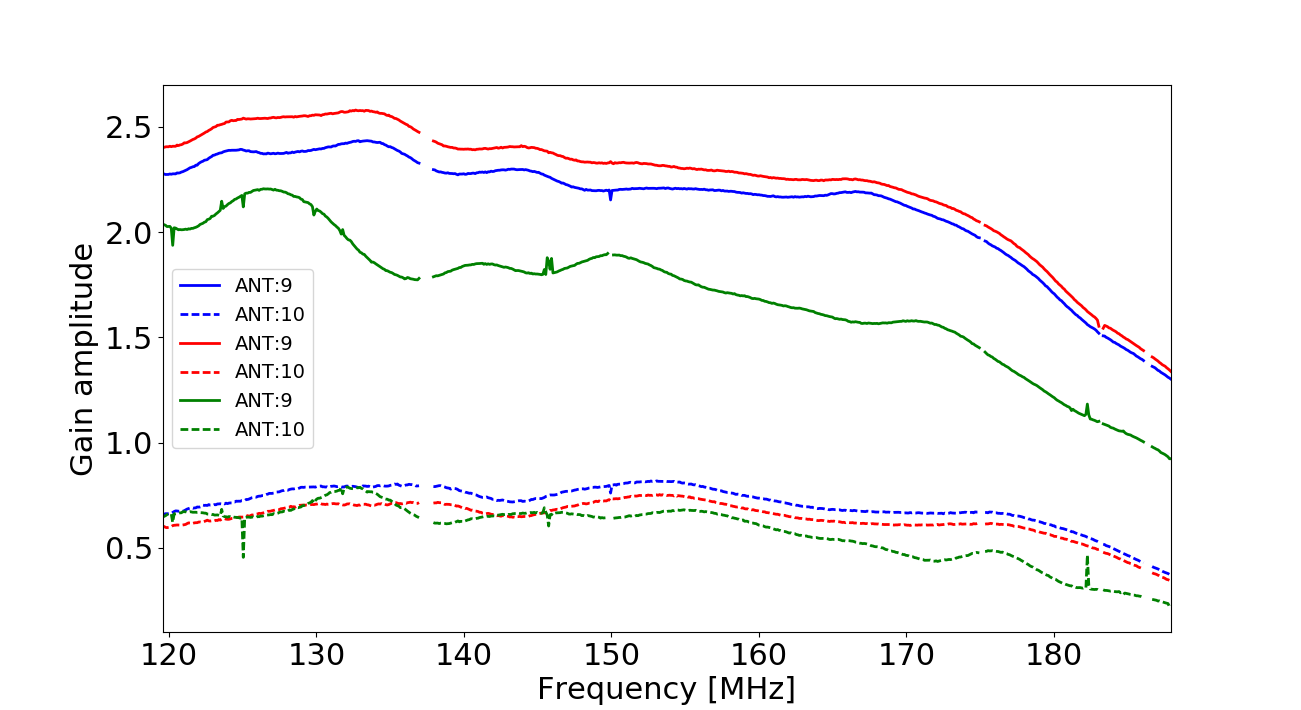
\includegraphics[width=0.47\linewidth]{bandpass_amp.png}%
%      \label{fig:evaluation:revenue}%
    }\qquad%
    \subfloat[Bandpass: Phase]{%
      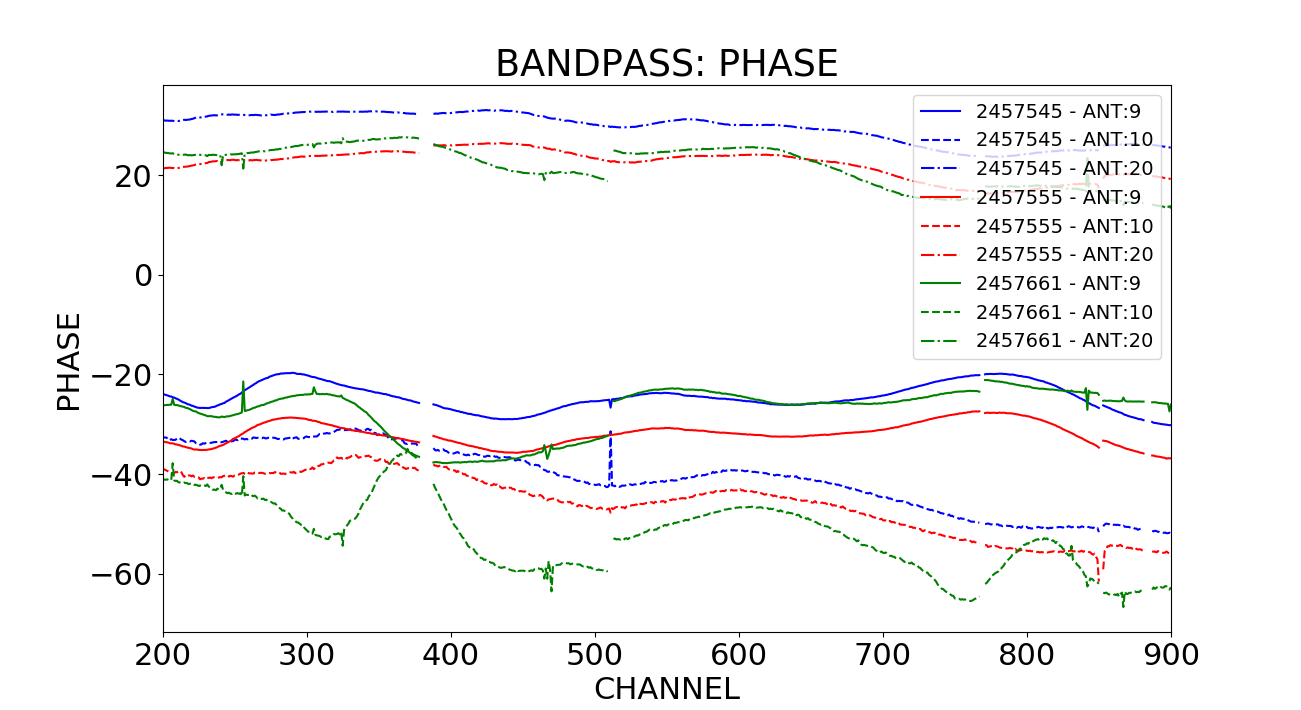
\includegraphics[width=0.47\linewidth]{bandpass_phase.png}%
%      \label{fig:evaluation:avgPrice}%
    }
    \caption{Bandpass gain solutions. {\bf (GB: plot only two antennas as it is too crowded. Try to make lines thicker as they are hard to see. Y title should be Gain amplitude. If you can plot both as a function of frequency would be better. Y title should be Gain phase (degrees). I would remove both plot titles.)}}
\label{fig:bandpass}
  \end{minipage}


Visibilities were then Fourier transformed and deconvolved using the CASA task {\it clean} (Figure~\ref{fig:gc_first_cal}).

\begin{center}\vspace{1cm}
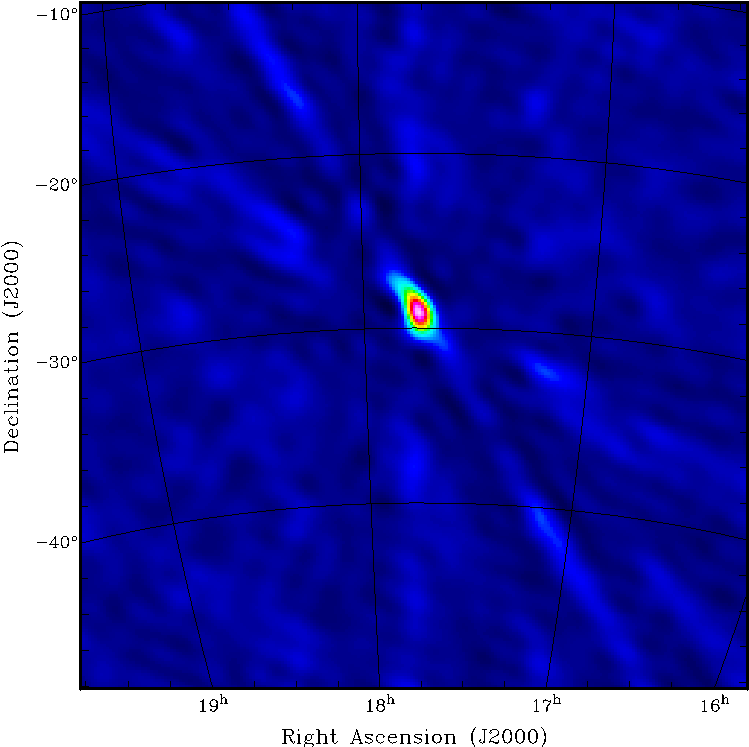
\includegraphics[width=0.4\linewidth]{gc_first_cal.png}
\captionof{figure}{\color{Green} The computed delays.}
\label{fig:gc_first_cal}
\end{center}\vspace{1cm}



\subsection*{Delay and Bandpass Calibration}
\begin{enumerate}
 \item Find the snapshot in which the Galactic center is closest to transit.
 \item Do a delay and bandpass calibration assuming a 1Jy point source model for the Galactic center.
 \item Apply gain solutions to all other snapshots.
\end{enumerate}
The computed delays seem to be quite stable as, even after ten days, there is almost no change in the delays. After $\sim$100 
days we see a bit more deviation, although not as much as one would expect.

The bandpass gain solutions are depicted below for a subset of antennas.
The phases are almost flat as the phase slope was removed by the delay calibration step. Again the bandpass 
gains also seem to be quite stable over time.


\subsection*{Absolute Flux Calibration}
\begin{enumerate}
 \item Find the snapshots containing the two flux calibrators (PMN J2101 2802 and PMN J2107 2526).
 \item Use Eq.~\eqref{eq:c} to obtain the correct scale factor.
 \item Apply scale factor to all other snapshots.
\end{enumerate}
The absolute flux calibration procedure we used is based on the following equation:
\begin{equation}
C = \frac{\sum_{kt}(B_{kt}^{\nu})^2\sum_k{M_{k}^{\nu}}}{\sum_{kt}B_{kt}^{\nu}S_{kt}^{\nu}},\label{eq:c}
\end{equation}
where $B_{kt}^{\nu}$ is the attenuation factor source $k$ experiences due to the primary beam at time $t$ and frequency $\nu$,
$S_{kt}^{\nu}$ is the measured uncalibrated apparent flux (not connected to the correct flux scale) of source $k$ at time $t$ and frequency $\nu$ and $M_{k}^{\nu}$ represents the 
intrinsic flux density of source $k$ at frequency $\nu$. 
Calibrated images of the delay and bandpass calibrator (Galactic Center) and the absolute flux calibrators (PMN J2101 2802 and PMN J2107 2526) is displayed in
the following two figures. 

\begin{minipage}{\columnwidth}
    \makeatletter
    \newcommand{\@captype}{figure}
    \makeatother
    \centering
    \subfloat[Delay and Bandpass Calibrator]{%
      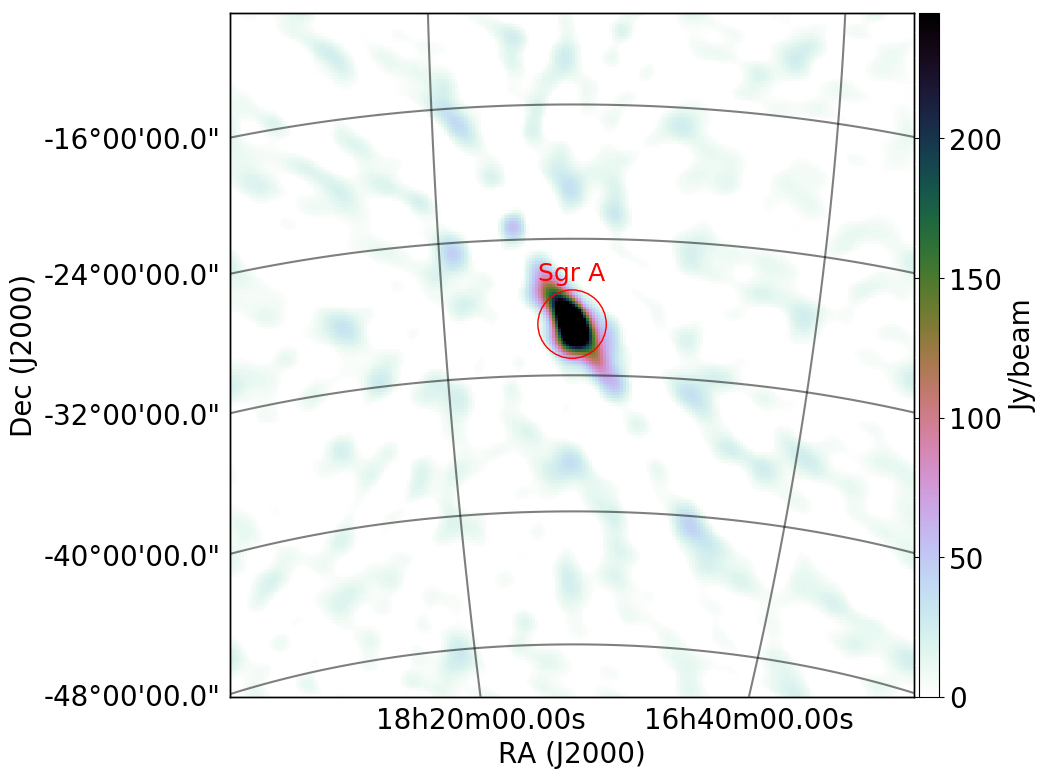
\includegraphics[width=0.47\linewidth]{GC.png}%
      \label{fig:evaluation:revenue}%
    }\qquad%
    \subfloat[Absolute Flux Calibrators]{%
      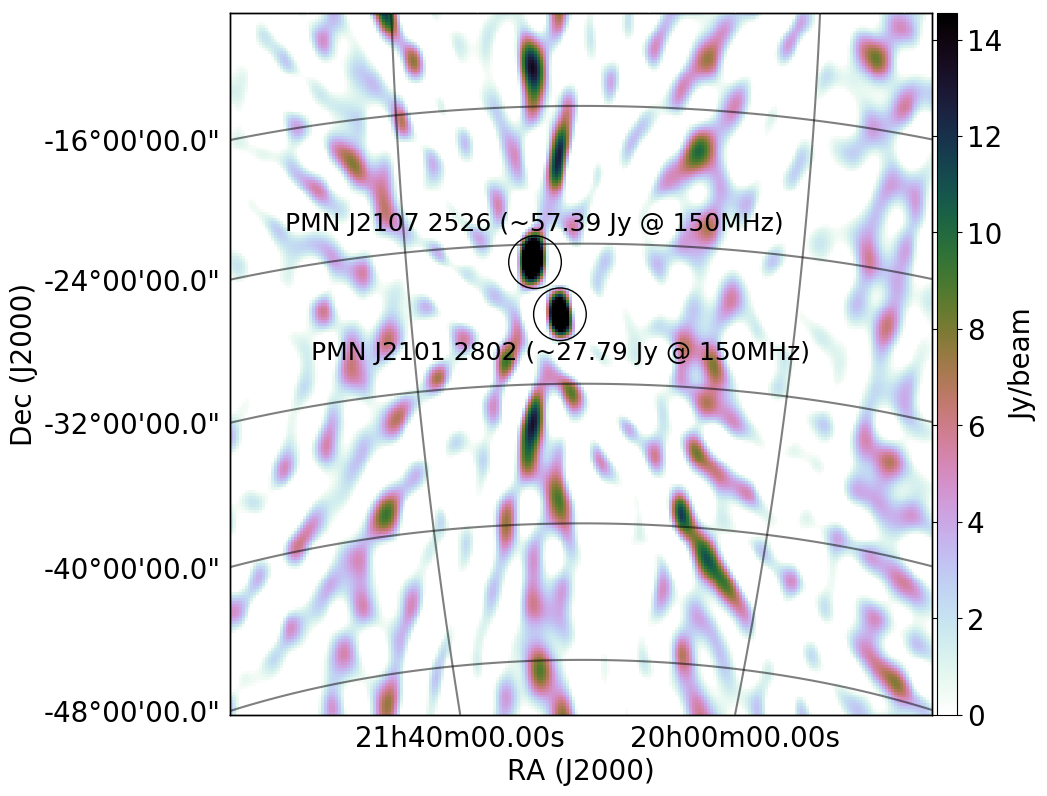
\includegraphics[width=0.47\linewidth]{ABS.png}%
      \label{fig:evaluation:avgPrice}%
    }
    \caption{\color{Green} Calibrators @ 150 MHz.}
  \end{minipage}
  
% \begin{table}
% \caption{The names and properties of the two absolute flux calibrators.\label{tab:sources}}
% \begin{center}
%   \begin{tabular}{ | c | c | c | c | c |}
%     \hline
%     Source Name & RA & DEC & $\sim$ $M^{150}$ & $M^{189}$\\ \hline\hline
%     PMN J2101 2802 & $21^h01^m37.7^s$ & $-28^{\circ}01'55''$ & 27.79 Jy & 23.1 Jy\\ 
%     PMN J2107 2526 & $21^h07^m25.3^s$ & $-25^{\circ}25'40''$ & 57.39 Jy & 47.7 Jy\\
%     \hline
%   \end{tabular}
% \end{center}
% \end{table}

\section*{HEALPIX}

The calibrated snapshots are projected and stitched together (using squared beam weighting) onto a HEALPIX map during the final step of the pipeline. The output HEALPIX map 
obtained by combining three entire Julian days worth or snapshots is seen below. The acronyms GC and ABS (visible in the figure below) respectively refer 
to the Galactic center and absolute flux calibrator fields

\begin{center}\vspace{1cm}
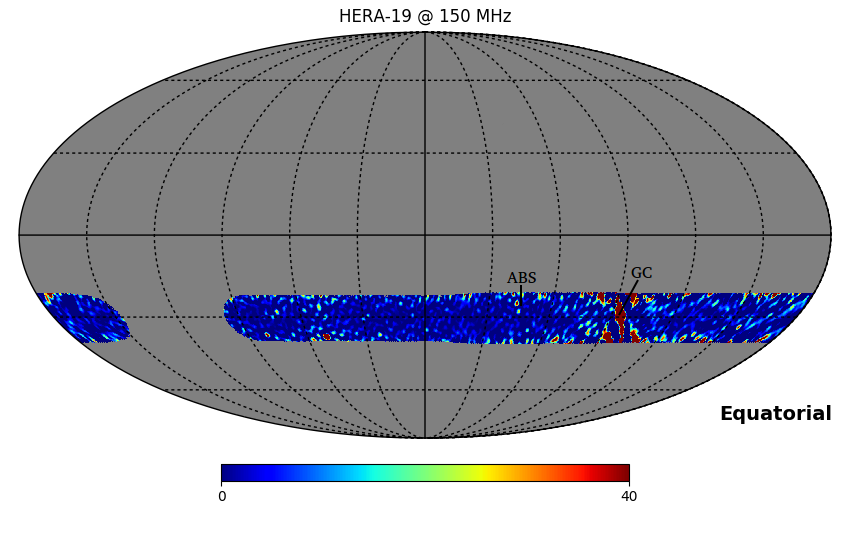
\includegraphics[width=1\linewidth]{ALL_SKY0.png}
\captionof{figure}{\color{Green} HERA-19 @ 150 MHz (2457545, 2457555 and 2457661). The units of the colorbar is Jy.}
\end{center}\vspace{1cm}


%\begin{center}\vspace{1cm}
%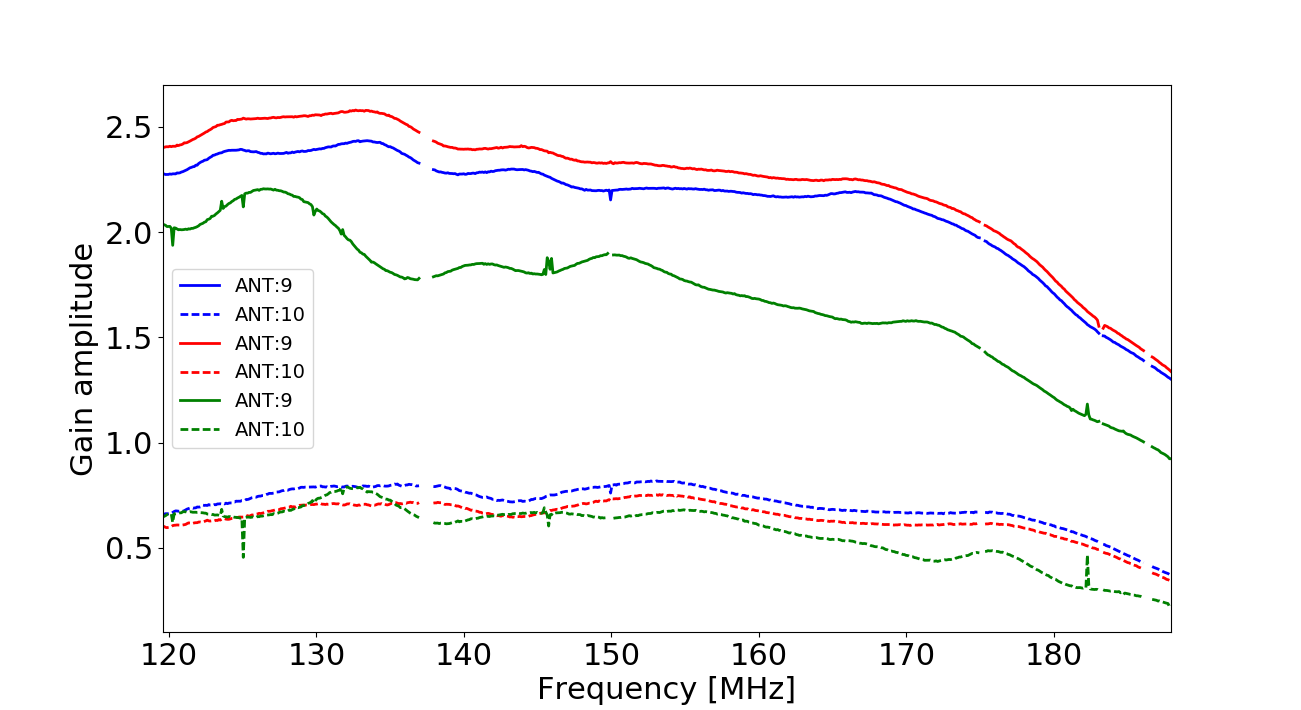
\includegraphics[width=1.0\linewidth]{bandpass_amp.png}
%\captionof{figure}{\color{Green} Figure caption}
%\end{center}\vspace{1cm}

%\begin{center}\vspace{1cm}
%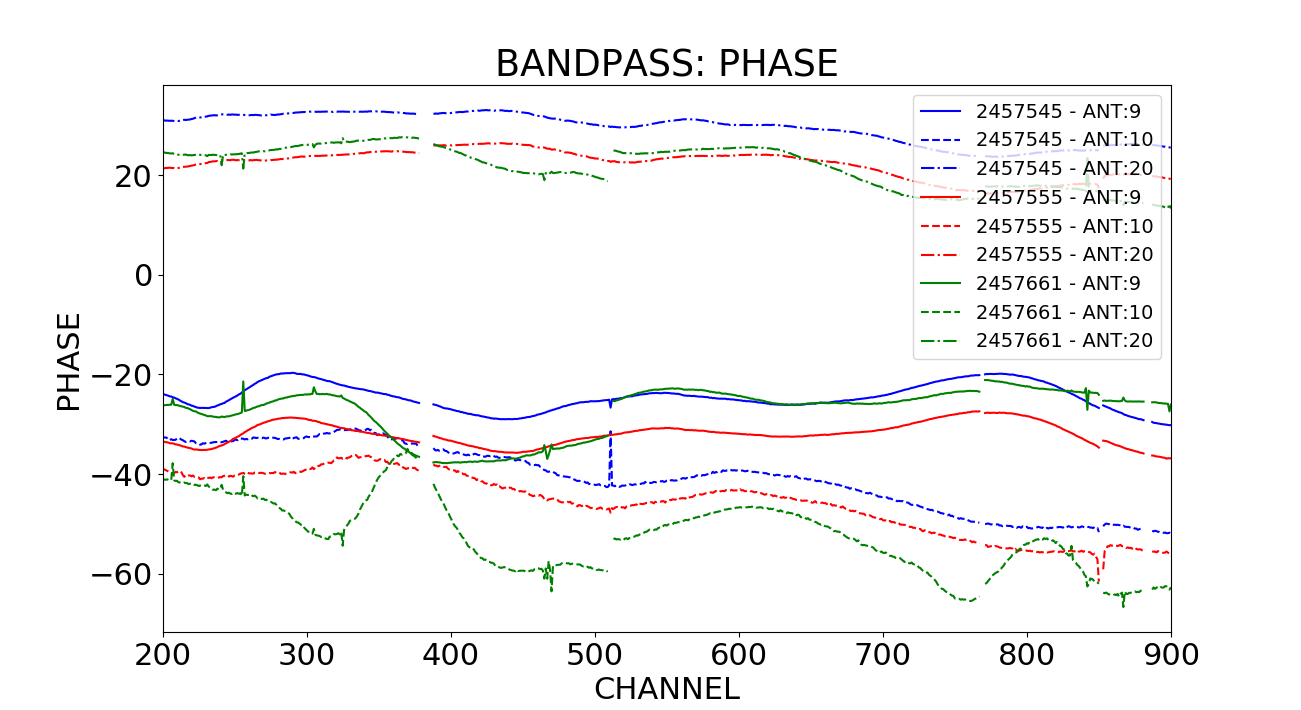
\includegraphics[width=1.0\linewidth]{bandpass_phase.png}
%\captionof{figure}{\color{Green} Figure caption}
%\end{center}\vspace{1cm}



%\section*{Main Objectives}

%\begin{enumerate}
%\item Lorem ipsum dolor sit amet, consectetur.
%\item Nullam at mi nisl. Vestibulum est purus, ultricies cursus volutpat sit amet, vestibulum eu.
%\item Praesent tortor libero, vulputate quis elementum a, iaculis.
%\item Phasellus a quam mauris, non varius mauris. Fusce tristique, enim tempor varius porta, elit purus commodo velit, pretium mattis ligula nisl nec ante.
%\item Ut adipiscing accumsan sapien, sit amet pretium.
%\item Estibulum est purus, ultricies cursus volutpat
%\item Nullam at mi nisl. Vestibulum est purus, ultricies cursus volutpat sit amet, vestibulum eu.
%\item Praesent tortor libero, vulputate quis elementum a, iaculis.
%\end{enumerate}

%----------------------------------------------------------------------------------------
%	MATERIALS AND METHODS
%----------------------------------------------------------------------------------------

%\section*{Materials and Methods}

%Fusce magna risus, molestie ut porttitor in, consectetur sed mi. Vestibulum ante ipsum primis in faucibus orci luctus et ultrices posuere cubilia Curae; Pellentesque consectetur blandit pellentesque. Sed odio justo, viverra nec porttitor vel, lacinia a nunc. Suspendisse pulvinar euismod arcu, sit amet accumsan enim fermentum quis. In id mauris ut dui feugiat egestas. Vestibulum ac turpis lacinia nisl commodo sagittis eget sit amet sapien.

%------------------------------------------------

%\subsection*{Mathematical Section}

%Nulla vel nisl sed mauris auctor mollis non sed. 

%\begin{equation}
%E = mc^{2}
%\label{eqn:Einstein}
%\end{equation}

%Curabitur mi sem, pulvinar quis aliquam rutrum. (1) edf (2)
%, $\Omega=[-1,1]^3$, maecenas leo est, ornare at. $z=-1$ edf $z=1$ sed interdum felis dapibus sem. $x$ set $y$ ytruem. 
%Turpis $j$ amet accumsan enim $y$-lacina; 
%ref $k$-viverra nec porttitor $x$-lacina. 

%Vestibulum ac diam a odio tempus congue. Vivamus id enim nisi:

%\begin{eqnarray}
%\cos\bar{\phi}_k Q_{j,k+1,t} + Q_{j,k+1,x}+\frac{\sin^2\bar{\phi}_k}{T\cos\bar{\phi}_k} Q_{j,k+1} &=&\nonumber\\ 
%-\cos\phi_k Q_{j,k,t} + Q_{j,k,x}-\frac{\sin^2\phi_k}{T\cos\phi_k} Q_{j,k}\label{edgek}
%\end{eqnarray}
%and
%\begin{eqnarray}
%\cos\bar{\phi}_j Q_{j+1,k,t} + Q_{j+1,k,y}+\frac{\sin^2\bar{\phi}_j}{T\cos\bar{\phi}_j} Q_{j+1,k}&=&\nonumber \\
%-\cos\phi_j Q_{j,k,t} + Q_{j,k,y}-\frac{\sin^2\phi_j}{T\cos\phi_j} Q_{j,k}.\label{edgej}
%\end{eqnarray} 

%Nulla sed arcu arcu. Duis et ante gravida orci venenatis tincidunt. Fusce vitae lacinia metus. Pellentesque habitant morbi. $\mathbf{A}\underline{\xi}=\underline{\beta}$ Vim $\underline{\xi}$ enum nidi $3(P+2)^{2}$ lacina. Id feugain $\mathbf{A}$ nun quis; magno.

%----------------------------------------------------------------------------------------
%	RESULTS 
%----------------------------------------------------------------------------------------

% \section*{Results}
% 
% Donec faucibus purus at tortor egestas eu fermentum dolor facilisis. Maecenas tempor dui eu neque fringilla rutrum. Mauris \emph{lobortis} nisl accumsan. Aenean vitae risus ante.
% %
% \begin{wraptable}{l}{12cm} % Left or right alignment is specified in the first bracket, the width of the table is in the second
% \begin{tabular}{l l l}
% \toprule
% \textbf{Treatments} & \textbf{Response 1} & \textbf{Response 2}\\
% \midrule
% Treatment 1 & 0.0003262 & 0.562 \\
% Treatment 2 & 0.0015681 & 0.910 \\
% Treatment 3 & 0.0009271 & 0.296 \\
% \bottomrule
% \end{tabular}
% \captionof{table}{\color{Green} Table caption}
% \end{wraptable}
% %
% Phasellus imperdiet, tortor vitae congue bibendum, felis enim sagittis lorem, et volutpat ante orci sagittis mi. Morbi rutrum laoreet semper. Morbi accumsan enim nec tortor consectetur non commodo nisi sollicitudin. Proin sollicitudin. Pellentesque eget orci eros. Fusce ultricies, tellus et pellentesque fringilla, ante massa luctus libero, quis tristique purus urna nec nibh.
% 
% Nulla ut porttitor enim. Suspendisse venenatis dui eget eros gravida tempor. Mauris feugiat elit et augue placerat ultrices. Morbi accumsan enim nec tortor consectetur non commodo. Pellentesque condimentum dui. Etiam sagittis purus non tellus tempor volutpat. Donec et dui non massa tristique adipiscing. Quisque vestibulum eros eu. Phasellus imperdiet, tortor vitae congue bibendum, felis enim sagittis lorem, et volutpat ante orci sagittis mi. Morbi rutrum laoreet semper. Morbi accumsan enim nec tortor consectetur non commodo nisi sollicitudin.
% 
% \begin{center}\vspace{1cm}
% \includegraphics[width=0.8\linewidth]{placeholder}
% \captionof{figure}{\color{Green} Figure caption}
% \end{center}\vspace{1cm}
% 
% In hac habitasse platea dictumst. Etiam placerat, risus ac.
% 
% Adipiscing lectus in magna blandit:
% 
% \begin{center}\vspace{1cm}
% \begin{tabular}{l l l l}
% \toprule
% \textbf{Treatments} & \textbf{Response 1} & \textbf{Response 2} \\
% \midrule
% Treatment 1 & 0.0003262 & 0.562 \\
% Treatment 2 & 0.0015681 & 0.910 \\
% Treatment 3 & 0.0009271 & 0.296 \\
% \bottomrule
% \end{tabular}
% \captionof{table}{\color{Green} Table caption}
% \end{center}\vspace{1cm}
% 
% Vivamus sed nibh ac metus tristique tristique a vitae ante. Sed lobortis mi ut arcu fringilla et adipiscing ligula rutrum. Aenean turpis velit, placerat eget tincidunt nec, ornare in nisl. In placerat.
% 
% \begin{center}\vspace{1cm}
% \includegraphics[width=0.8\linewidth]{placeholder}
% \captionof{figure}{\color{Green} Figure caption}
% \end{center}\vspace{1cm}
% 
% %----------------------------------------------------------------------------------------
% %	CONCLUSIONS
% %----------------------------------------------------------------------------------------
% 
% \color{SaddleBrown} % SaddleBrown color for the conclusions to make them stand out
% 
% \section*{Conclusions}
% 
% \begin{itemize}
% \item Pellentesque eget orci eros. Fusce ultricies, tellus et pellentesque fringilla, ante massa luctus libero, quis tristique purus urna nec nibh. Phasellus fermentum rutrum elementum. Nam quis justo lectus.
% \item Vestibulum sem ante, hendrerit a gravida ac, blandit quis magna.
% \item Donec sem metus, facilisis at condimentum eget, vehicula ut massa. Morbi consequat, diam sed convallis tincidunt, arcu nunc.
% \item Nunc at convallis urna. isus ante. Pellentesque condimentum dui. Etiam sagittis purus non tellus tempor volutpat. Donec et dui non massa tristique adipiscing.
% \end{itemize}
% 
% \color{DarkSlateGray} % Set the color back to DarkSlateGray for the rest of the content
% 
% %----------------------------------------------------------------------------------------
% %	FORTHCOMING RESEARCH
% %----------------------------------------------------------------------------------------
% 
% \section*{Forthcoming Research}
% 
% Vivamus molestie, risus tempor vehicula mattis, libero arcu volutpat purus, sed blandit sem nibh eget turpis. Maecenas rutrum dui blandit lorem vulputate gravida. Praesent venenatis mi vel lorem tempor at varius diam sagittis. Nam eu leo id turpis interdum luctus a sed augue. Nam tellus.

 %----------------------------------------------------------------------------------------
%	REFERENCES
%----------------------------------------------------------------------------------------

\nocite{*} % Print all references regardless of whether they were cited in the poster or not
\bibliographystyle{plain} % Plain referencing style
\bibliography{sample} % Use the example bibliography file sample.bib

\begin{center}\vspace{1cm}

\includegraphics[width=0.35\linewidth]{ska_logo.jpg}
\end{center}\vspace{1cm}

%----------------------------------------------------------------------------------------
%	ACKNOWLEDGEMENTS
%----------------------------------------------------------------------------------------

% \section*{Acknowledgements}
% 
% Etiam fermentum, arcu ut gravida fringilla, dolor arcu laoreet justo, ut imperdiet urna arcu a arcu. Donec nec ante a dui tempus consectetur. Cras nisi turpis, dapibus sit amet mattis sed, laoreet.

%----------------------------------------------------------------------------------------

\end{multicols}
\end{document}
